%%%% utfpr-poster.tex, 2019/12/01
%%%% Copyright (C) 2018-2019 Luiz E. M. Lima (luizeduardomlima@gmail.com)
%%
%% This work may be distributed and/or modified under the conditions of the
%% LaTeX Project Public License, either version 1.3 of this license or (at your
%% option) any later version.
%% The latest version of this license is in
%%   http://www.latex-project.org/lppl.txt
%% and version 1.3 or later is part of all distributions of LaTeX version
%% 2005/12/01 or later.
%%
%% This work has the LPPL maintenance status `maintained'.
%%
%% The Current Maintainer of this work is Luiz E. M. Lima.
%%
%% This work consists of the files utfpr-poster.sty and utfpr-poster.tex.
%%
%% A brief description of this work is in readme.txt.

%% Detecção e aviso sobre comandos obsoletos
% \RequirePackage[l2tabu, orthodox]{nag}

%% Classe de documento e opções
\documentclass[%% Opções: [>] passada para pacotes
  final,%% Em oposição à de rascunho (draft) [>]
  english,%% Idioma secundário (penúltimo) [>]
  brazilian,%% Idioma primário (último) [>]
]{beamer}

%% Pacotes utilizados
\usepackage[%% Opções: [>] passada para beamerposter
  Times   = false,%% Fontes Times (roman) e Arial (sans serif): true ou false
  BibURLs = false,%% Links de URLs nas referências: true ou false
  ABNTNum = none,%% Estilo numérico ABNT: none (AUTOR, ANO), dflt (1) e brkt [1]
  size    = custom,%% Tamanho de papel: a0, a1, a2, a3, a4 e custom [>]
  width   = 90,%% Largura de papel em centímetros (custom) [>]
  height  = 120,%% Altura de papel em centímetros (custom) [>]
  scale   = 1.5,%% Escala de fontes [>]
]{utfpr-poster}

%% Arquivo de referências
\addbibresource{utfpr-poster.bib}

%% Informações do documento
%%%% Título
\title{%
  Here's a good title, check it out
}
%%%% Assunto
\subject{Nome e/ou Sigla do Congresso, Seminário ou Evento Técnico/Científico}
%%%% Autor(es)
\author{%
  Primeiro(a)~M.~Autor(a)\inst{1}%
  \orcidlinkicon{0000-0000-0000-0001}%
  \and Segundo(a)~M.~Autor(a)\inst{2}%
  \orcidlinkicon{0000-0000-0000-0002}%
  \and Terceiro(a)~M.~Autor(a)\inst{3}%
  \orcidlinkicon{0000-0000-0000-0003}%
  \and\\Quarto(a)~M.~Autor(a)\inst{4}%
  \orcidlinkicon{0000-0000-0000-0004}%
  \and Quinto(a)~M.~Autor(a)\inst{5}%
  \orcidlinkicon{0000-0000-0000-0005}%
}
%%%% Instituição(ões) e e-mail(s)
\institute{%
  \affil[1,3,5]{\utfprname, Ponta Grossa, Paraná, Brasil}%
  \and\affil[2,4]{Instituição do(a) Autor(a) Externo(a), Cidade, Estado, País}%
  \and\email[1]{autor1@dominio}%
  \sep\email[2]{autor2@dominio}%
  \sep\email[3]{autor3@dominio}%
  \sep\email[4]{autor4@dominio}%
  \sep\email[5]{autor5@dominio}%
}
%%%% Data: comente para gerar a data atual
\date{}

%% Início do documento
\begin{document}

\begin{frame}[t, fragile = singleslide]

\begin{columns}[t, onlytextwidth]%% Início do cabeçalho
%
\begin{column}{0.1\textwidth}
\begin{flushleft}

\includegraphics[width = \columnwidth]{./Logos/evento}%% Logomarca superior-esquerdo
\vspace*{0.5\baselineskip}

\includegraphics[width = \columnwidth]{./Logos/evento-org}%% Logomarca inferior-esquerdo
\end{flushleft}
\end{column}
%
\begin{column}{0.8\textwidth}
\titlepage%
\end{column}
%
\begin{column}{0.1\textwidth}
\begin{flushright}

\includegraphics[width = \columnwidth]{./Logos/utfpr-pg}%% Logomarca superior-direito
\vspace*{0.5\baselineskip}

\includegraphics[width = \columnwidth]{./Logos/inst-ext}%% Logomarca inferior-direito
% \vspace*{0.5\baselineskip}
% \meclogo%% Logomarca do Ministério da Educação
% \vspace*{0.5\baselineskip}
% \govlogo%% Logomarca do Governo Federal
\end{flushright}
\end{column}
%
\end{columns}%% Fim do cabeçalho

\begin{columns}[t, onlytextwidth]
%
\begin{column}{0.49\textwidth}
%
\begin{block}{INTRODUÇÃO}
\begin{itemize}
\item Este poster foi desenvolvido com base na classe \href{http://www.ctan.org/pkg/beamer/}{\LaTeX/Beamer~\linkicon}, usando o pacote \LaTeX\ \enquote{\href{http://ctan.org/pkg/beamerposter/}{beamerposter~\linkicon}}.
\item Exemplos de referências podem ser observados nas citações:
\begin{itemize}
\item Implícita: \ldots\ \cite{Lamport1994,VanEkenstein1997}.
\item Explícita: Segundo \textcite{Wizentier1992},\ldots
\end{itemize}
\item Citações e referências podem ser inseridas neste documento usando os comandos do pacote \LaTeX\ \enquote{\href{http://ctan.org/pkg/biblatex/}{biblatex~\linkicon}}.
\item Os dados de cada referência podem ser obtidos de um arquivo \enquote{bibtex} (*.bib), geralmente na própria página de \textit{download} da referência (artigos, livros, etc.), ou no Google Acadêmico, etc.
\item Para gerar ou editar entradas de arquivos \enquote{bibtex} (*.bib), pode-se utilizar a ferramenta \enquote{\href{http://truben.no/latex/bibtex/}{Bibtex Editor~\linkicon}} ou \enquote{\href{http://zbib.org/}{ZoteroBib~\linkicon}}, entre outras.
\end{itemize}
\end{block}
%
\begin{block}{REVISÃO DA LITERATURA}
Exemplo de lista de itens numerada:
\begin{enumerate}
\item Item numerado 1.
\item Item numerado 2.
\item Item numerado 3.
\item Item numerado 4.
\item Item numerado 5.
\end{enumerate}
Uma equação como $y = a x^2 + b x + c$ pode ser inserida ao longo do texto de um parágrafo usando o ambiente \LaTeX\ \enquote{math} (\verb|$...$|).
Por outro lado, a seguinte equação é um exemplo de equação não numerada inserida numa linha em separado usando o ambiente \LaTeX\ \enquote{displaymath} (\verb|\[...\]|).
\[
\frac{\mathrm{d} y}{\mathrm{d} x} = \gamma \operatorname{sen} x
\]
A Eq.~\eqref{eq:fx} é um exemplo de equação inserida usando o ambiente \LaTeX\ \enquote{equation} e numerada automaticamente.
\begin{equation}\label{eq:fx}
f(x) = \frac{1}{\alpha} \int_0^L \left(\frac{x^2}{2} - \frac{x^3}{3}\right) \mathrm{d} x
\end{equation}
Para gerar ou editar equações em \LaTeX, pode-se utilizar a ferramenta \enquote{\href{http://formulasheet.com/}{Formula Sheet~\linkicon}}, entre outras.
\end{block}
%
\end{column}
%
\begin{column}{0.49\textwidth}
%
\begin{block}{MATERIAL E MÉTODOS}
A Fig.~\ref{fig:campuspontagrossa} é um exemplo de figura inserida usando o ambiente \LaTeX\ \enquote{figure} e numerada automaticamente.
\begin{figure}[!htb]
\centering%
\caption{Câmpus Ponta Grossa da UTFPR.}%
\label{fig:campuspontagrossa}
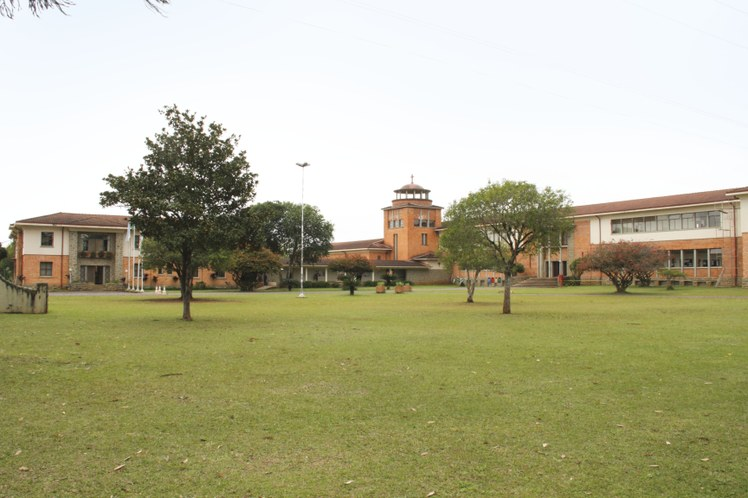
\includegraphics[width = 0.5\columnwidth]{./Figuras/campuspontagrossa}
\source{\textcite{UTFPR2018}.}
\end{figure}
A Tab.~\ref{tab:Ldimens} é um exemplo de tabela inserida usando o ambiente \LaTeX\ \enquote{table} e numerada automaticamente.
\begin{table}[!htb]
\centering%
\small%
\caption{Exemplo de legenda de tabela.}%
\label{tab:Ldimens}
\begin{tabular*}{\columnwidth}{@{\extracolsep{\fill}}llll}
\toprule
$L$   & $L^2$     & $L^3$     & $L^4$     \\
{[m]} & {[m$^2$]} & {[m$^3$]} & {[m$^4$]} \\
\midrule
1     & 1         & 1         & 1         \\
2     & 4         & 8         & 16        \\
3     & 9         & 27        & 81        \\
4     & 16        & 64        & 256       \\
5     & 25        & 125       & 625       \\
\bottomrule
\addlinespace
\end{tabular*}
\source{autoria própria.}
\end{table}
Para gerar ou editar tabelas em \LaTeX, pode-se utilizar a ferramenta \enquote{\href{http://www.tablesgenerator.com/}{Tables Generator~\linkicon}}, entre outras.
\par%
Informações e dicas sobre \TeX/\LaTeX\ podem ser obtidas em:
\begin{itemize}
\item \href{http://www.latex-project.org/}{\LaTeX\ Project~\linkicon}.
\item \href{http://www.ctan.org/}{Comprehensive \TeX\ Archive Network (CTAN)~\linkicon}.
\item \href{http://www.tug.org/}{\TeX\ Users Group (TUG)~\linkicon}.
\item \href{http://en.wikibooks.org/wiki/LaTeX/}{\LaTeX\ --- Wikibooks~\linkicon}.
\item \href{http://tex.stackexchange.com/}{\TeX-\LaTeX\ Stack Exchange~\linkicon}.
\end{itemize}
\end{block}
%
\end{column}
%
\end{columns}

\begin{columns}[t, onlytextwidth]
%
\begin{column}{\textwidth}
%
\begin{block}{RESULTADOS E DISCUSSÃO}
As Figs.~\ref{fig:graficoxy1} a~\ref{fig:mapacampus} são mais exemplos de figuras inseridas usando o ambiente \LaTeX\ \enquote{figure} e dispostas em três colunas.
\begin{column}[T]{0.33\textwidth}
\begin{figure}[!htb]
\centering%
\caption{Exemplo de legenda de figura.}%
\label{fig:graficoxy1}
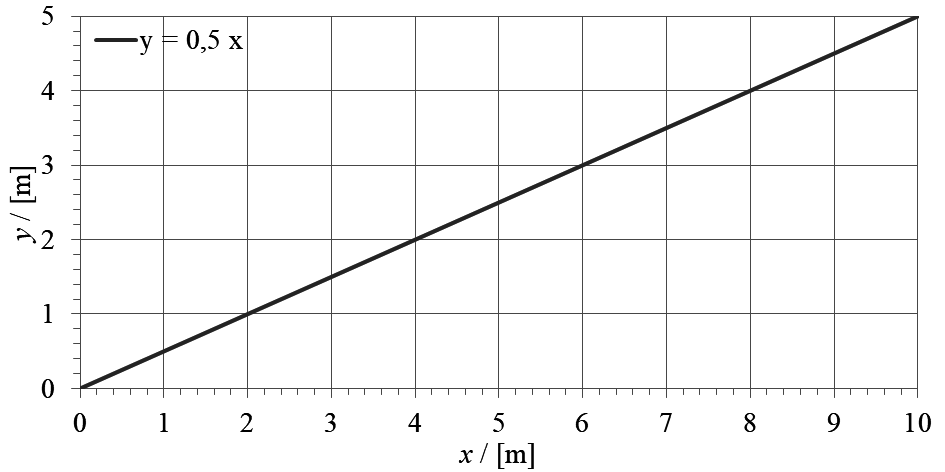
\includegraphics[height = 130mm]{./Figuras/graficoxy}
\source{autoria própria.}
\end{figure}
\end{column}
\yellowvrule%
\begin{column}[T]{0.33\textwidth}
\begin{figure}[!htb]
\centering%
\caption{Exemplo de legenda de figura.}%
\label{fig:graficoxy2}
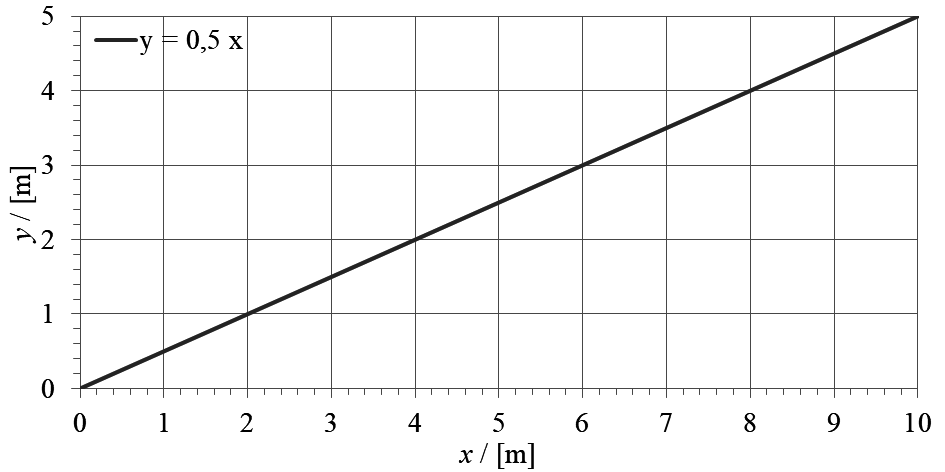
\includegraphics[height = 130mm]{./Figuras/graficoxy}
\source{autoria própria.}
\end{figure}
\end{column}
\yellowvrule%
\begin{column}[T]{0.33\textwidth}
\begin{figure}[!htb]
\centering%
\caption{Mapa com a localização dos câmpus da UTFPR.}%
\label{fig:mapacampus}
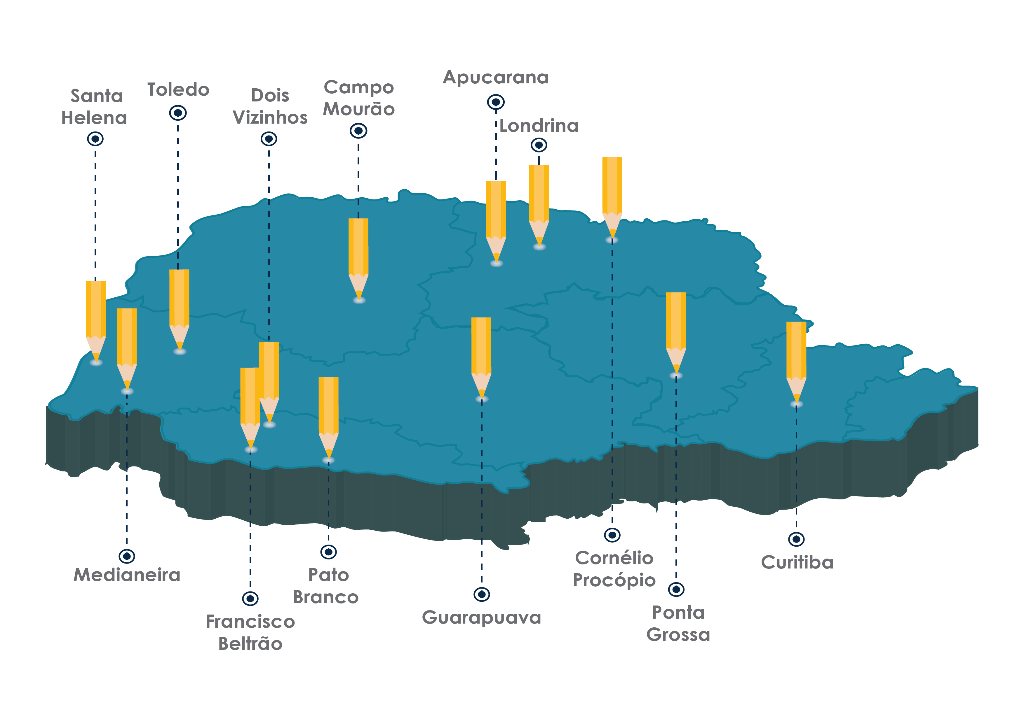
\includegraphics[height = 130mm]{./Figuras/mapacampus}
\source{\textcite{UTFPR2018}.}
\end{figure}
\end{column}
\end{block}
%
\end{column}
%
\end{columns}

\begin{columns}[t, onlytextwidth]
%
\begin{column}{0.49\textwidth}
%
\begin{block}{CONCLUSÕES}
\begin{itemize}
\item Conclusão 1.
\item Conclusão 2.
\item Conclusão 3.
\item Conclusão 4.
\item Conclusão 5.
\end{itemize}
\end{block}
%
\begin{block}{AGRADECIMENTOS}
\footnotesize%
Às organizações de fomento, pelo apoio recebido para o desenvolvimento deste trabalho e a participação neste evento:
\vfill%

\includegraphics[height = 20mm]{./Logos/apoio-capes}
\hspace*{5mm}

\includegraphics[height = 20mm]{./Logos/apoio-cnpq}
\hspace*{5mm}

\includegraphics[height = 20mm]{./Logos/apoio-fa-gov-pr}
\hspace*{5mm}

\includegraphics[height = 20mm]{./Logos/utfpr}
\end{block}
%
\end{column}
%
\begin{column}{0.49\textwidth}
%
\begin{block}{REFERÊNCIAS}
\printbibliography[heading = none]
\end{block}
%
\end{column}
%
\end{columns}

\vspace*{\stretch{1000}}

\begin{columns}[b]
%
\begin{column}{0.49\textwidth}
\respnotice[Declaração de Responsabidade]{o(s) autor(es) é(são) o(s) único(s) responsável(eis) pelas informações contidas neste documento.}
\end{column}
%
\begin{column}{0.49\textwidth}
\begin{flushright}

\includegraphics[height = 20mm]{./Logos/utfpr-110anos}%% Logomarca comemorativa da UTFPR (110 anos)
\hspace*{5mm}

\includegraphics[height = 20mm]{./Logos/utfpr-pg}%% Logomarca da UTFPR-PG
% \hspace*{5mm}
% \meclogobottom%% Logomarca do Ministério da Educação
% \hspace*{5mm}
% \govlogobottom%% Logomarca do Governo Federal
\end{flushright}
\end{column}
%
\end{columns}

\vspace*{\baselineskip}

\end{frame}

%% Fim do documento
\end{document}
